\documentclass[mathserif, aspectratio=169]{beamer}
%
%%%%%%%%%%%%%%%%%%%%%%%%%%%%%%%%%%%%%%%%%%%%%%%%%%%%%%%%%%%%%%%%%%%%%%%%
% need to split the includes to make spell checking work.
\usepackage{arev, arevmath}
\usepackage[scaled]{cabin}
\usepackage[T1]{fontenc}
\usepackage[super]{nth}
\usepackage{pifont}
\usepackage{wasysym}
\usepackage{tabularx}
\usepackage{array}
\usepackage{booktabs}
\usepackage{boldline}
\usepackage{colortbl}
%\usepackage{amsmath}
\usepackage{bm}
\usepackage{tcolorbox}
\usepackage{adjustbox}
\usepackage{minibox}
\usepackage{makecell}
\usepackage{adjustbox}
\usepackage{textcomp}
\usepackage[absolute,overlay]{textpos}
\setlength{\TPHorizModule}{1mm}%
\setlength{\TPVertModule}{1mm}%
\tcbuselibrary{skins}

\makeatletter
\newcommand{\antsize}{\@setfontsize{\antsize}{4pt}{4pt}}
\makeatother
\newcommand{\at}{\makeatletter @\makeatother}

\newcommand{\cmark}{\ding{51}}%
\newcommand{\bottomline}[1]{\vskip0pt plus 1fill{\alert{#1}\phantom{g}\vskip 1.0mm}}

\newcommand{\Quote}[2]{%
	\begin{center} 
		\begin{minipage}{0.7\textwidth} 
			\hrule
			\vskip 3mm
			\emph{{\color{ICTPblue} ``#1''}
			
			~~~~ {\color{ICTPorange} --- #2}}
			\vskip 3mm
			\hrule
			\vskip 2mm
		\end{minipage}
	\end{center}}


\mode<presentation>%
{
	\usetheme{default}
	%\usetheme[width=2.5cm]{PaloAlto}
	\usecolortheme{dove}
	\useoutertheme{infolines}
	% oder auch nicht

	% ICTP Colors
	\definecolor{ICTPblue}{RGB}{37,86,162} % 0x255682
	\definecolor{ICTPorange}{RGB}{255,130,0} % 0xff8200
	\definecolor{ICTPgreen}{RGB}{0,100,0}
	\definecolor{ICTPdark}{RGB}{80,80,80} % 0x505050
	\definecolor{ICTPlight}{RGB}{120,120,120}
	\definecolor{ICTPbrown}{RGB}{178,91,0}

	\definecolor{codebg}{rgb}{0.95,0.95,0.95}

	% Color theme
	\setbeamercolor{alerted text}{fg=ICTPorange}
	\setbeamercolor{frametitle}{fg=ICTPblue}
	\setbeamercolor{title}{fg=ICTPblue}
	\setbeamercolor{subtitle}{fg=ICTPorange}
	\setbeamercolor{normal text}{fg=ICTPdark}
	\setbeamercolor{author in foot}{fg=ICTPblue}
	\setbeamercolor{item}{fg=ICTPblue}
	\setbeamercolor{footline}{fg=ICTPblue}
	%\setbeamercolor{item projected}{bg=ICTPorange}
	%\setbeamercolor{item projected}{fg=white}

	\setbeamertemplate{headline}
	{}
	\setbeamertemplate{frametitle}
	{
		%\textbf{{\insertframetitle\phantom{g}}}\\
		%\textbf{\insertframetitle\phantom{g}}\\
		\textbf{\underline{\insertframetitle\phantom{g}}}\\
		%\textbf{\underline{\insertframetitle}}\\
		\vskip 1.0mm
		%{\color{UOLgold}\hrule height 2pt}
		%\par
	}
	\addtobeamertemplate{frametitle}{}{\vspace{-1em}}
	\setbeamertemplate{footline}{
		{%
			\textbf{ \hskip 3.0mm\insertshorttitle\phantom{.}---\phantom{.}\insertshortinstitute\hfill\insertframenumber\,/\,\inserttotalframenumber\hskip 3.0mm} 
		}
	}

	\setbeamertemplate{navigation symbols}{}%remove navigation symbols
	\setbeamertemplate{itemize items}[circle]
	\setbeamertemplate{enumerate items}[fg=ICTPblue]
	\setbeamercolor{itemize items}{fg=ICTPblue}
	\setbeamercolor{sidebar}{bg=ICTPblue}
	\setbeamercolor{title in sidebar}{fg=ICTPorange}
	\setbeamercolor{author in sidebar}{fg=ICTPorange}
	\setbeamercolor{section in sidebar}{fg=ICTPorange}
}

%\input{tikz/common-styles}

\usepackage{graphicx}
\usepackage[latin1]{inputenc}

\graphicspath{{../figs/}{../figs/common/}{../figs/islr/}}

\title[Statistical Learning] % (optional, nur bei langen Titeln n�tig)
{\textbf{Introduction to Statistical Learning\\ {\it with applications in Python}}\\%
		\href{www.statlearning.com}%
		{\tiny\it Based on ``Introduction to Statistical Learning, with applications in R'' by Gareth James, Daniela Witten, Trevor Hastie, Robert Tibishirani}\vspace{2em}}
		\vspace{-2.5cm}{}


		\author{\href{mailto:?to=Kurt Rinnert <kurt.rinnert@cern.ch>&subject=PWF Statistical Learning}{Kurt Rinnert}}

\institute[{\href{https://www.ictp.it/physics-without-frontiers.aspx}{Physics Without Frontiers} --- \href{https://www.ictp.it/}{ICTP}}] % (optional)
{\color{ICTPblue}\bfseries \href{https://www.ictp.it/physics-without-frontiers.aspx}{Physics Without Frontiers}\\\vspace{1mm}%
\href{https://www.ictp.it/}{
\includegraphics[width=0.20\textwidth]{common/ICTP-logo-full-trans.png}}\\%
\href{https://www.liverpool.ac.uk/physics/}{
\includegraphics[width=0.2\textwidth]{common/uol_logo.png}}}

\date{}

\titlegraphic{
	\texorpdfstring{\vspace{-2.8cm}}{}
	 \begin{minipage}[b][1.3cm][b]{0.26\textwidth}\color{ICTPlight}\antsize
		Copyright \textcopyright~2019\\
		\href{mailto:?to=Kurt Rinnert <kurt.rinnert@cern.ch>&subject=PWF Statistical Learning}{Kurt Rinnert <kurt.rinnert{\tt @}cern.ch>},
		\href{mailto:?to=Kate Shaw <kshaw@ictp.it>&subject=PWF Statistical Learning}{Kate Shaw <kshaw{\tt @}ictp.it>}\\
		Copying and distribution of this file, with or without modification,
		are permitted in any medium without royalty provided the copyright
		notice and this notice are preserved.  This file is offered as-is,
		without any warranty.


		Some of the figures in this presentation are taken from ``An Introduction to
		Statistical Learning, with applications in R''  (Springer, 2013) with
		permission from the authors: G. James, D. Witten,  T. Hastie and R. Tibshirani 
	 \end{minipage}\hspace{10cm}
}


\addtocounter{framenumber}{-1}

% nicer table row separation
\renewcommand{\arraystretch}{1.2}

% color boxes
\newcommand{\tabboxset}{\tcbset{enhanced, nobeforeafter, boxrule=0pt, boxsep=0pt, colback=codebg, colframe=codebg, coltext=ICTPdark, rounded corners, arc=4pt, fonttitle={\bfseries\tiny}}}
\newcommand{\codeboxset}{\tcbset{enhanced, nobeforeafter, boxrule=0pt, boxsep=0pt, colback=codebg, colframe=codebg, coltext=ICTPdark, rounded corners, arc=4pt, fonttitle={\bfseries\tiny}}}

\newcommand{\orange}{\color{ICTPorange}}
\newcommand{\blue}{\color{ICTPblue}}
\newcommand{\dark}{\color{ICTPdark}}
\newcommand{\R}{\mathbb{R}}
\newcommand{\dat}[1]{{\footnotesize\tt\orange #1}}
\newcommand{\e}[1]{\emph{#1}}
\newcommand{\bh}{\hat{\beta}}
\newcommand{\h}{\hat}

\makeatletter
\newcommand{\includegraphicsdpi}[3]{%
	\pdfimageresolution=#1%
	\includegraphics[#2]{#3}%
	\pdfimageresolution=72%
}

\newenvironment{blurb}%
	{\begin{center}\begin{minipage}{0.6\textwidth}\footnotesize}
	{\end{minipage}\end{center}}

\newenvironment{cpage}%
	{\begin{center}\begin{minipage}{0.75\textwidth}}
	{\end{minipage}\end{center}}

\newenvironment{popblock}[2]%
	{\begin{center}\begin{minipage}{#1}\footnotesize
		\begin{tcolorbox}[colframe=codebg, colback=white, colupper=ICTPdark, title={\normalsize\bfseries\blue #2}]}
	{\end{tcolorbox}\end{minipage}\end{center}}
\makeatother

\subtitle{\bfseries%
  {Linear Regression, Part 3}\\%
  {\tiny\it qualitative predictors, interaction \& non-linear extensions, outliers, collinearity}\\%
}
\begin{document}
\frame[plain]{
	\vskip 1.0mm
	\titlepage
	\vskip 1.0mm
}


\begin{frame}{Abstract}

	\begin{blurb}
		Linear models are an important topic in statistical learning.  

		The true relationships between predictors and responses are rarely linear.
		But linear models often provide reasonable approximation. They provide
		high interpretability and have low variance, mitigating the risk of over-fitting.
		Linear models can be extended to include (some) non-linear relationships. 

		Linear models also provide an excellent baseline to compare other models against: if 
		our sophisticated model does not do much better than a linear model we might consider
		trading some bias for lower variance.
	\end{blurb}
\end{frame}

\begin{frame}{Overview}
	\begin{itemize}
		\item Qualitative versus quantitative predictors.
		\item Interactions among predictors.
		\item Non-linear extensions to the linear model.
		\item Outliers \& high leverage points.
		\item Collinearity.
	\end{itemize}
	\bottomline{This will conclude our long journey through linear regression.}
\end{frame}

\begin{frame}{Example: Credit Data Set}
	\begin{columns}
		\begin{column}{0.5\textwidth}
			\begin{itemize}
				\item The plot on the right shows the \e{quantitative} variables
					in the data set.
				\item The dataset also contains \e{qualitative} predictors:
				\item[] \dat{gender}: \val{Male}, \val{Female}
				\item[] \dat{married}: \val{Yes}, \val{No}
				\item[] \dat{student}: \val{Yes}, \val{No}
				\item[] \dat{ethnicity}: \val{Asian}, \val{African American}, \val{Caucasian}
			\end{itemize}
		\end{column}
		\begin{column}{0.5\textwidth}
			\vspace{-10mm}
			\begin{center}
				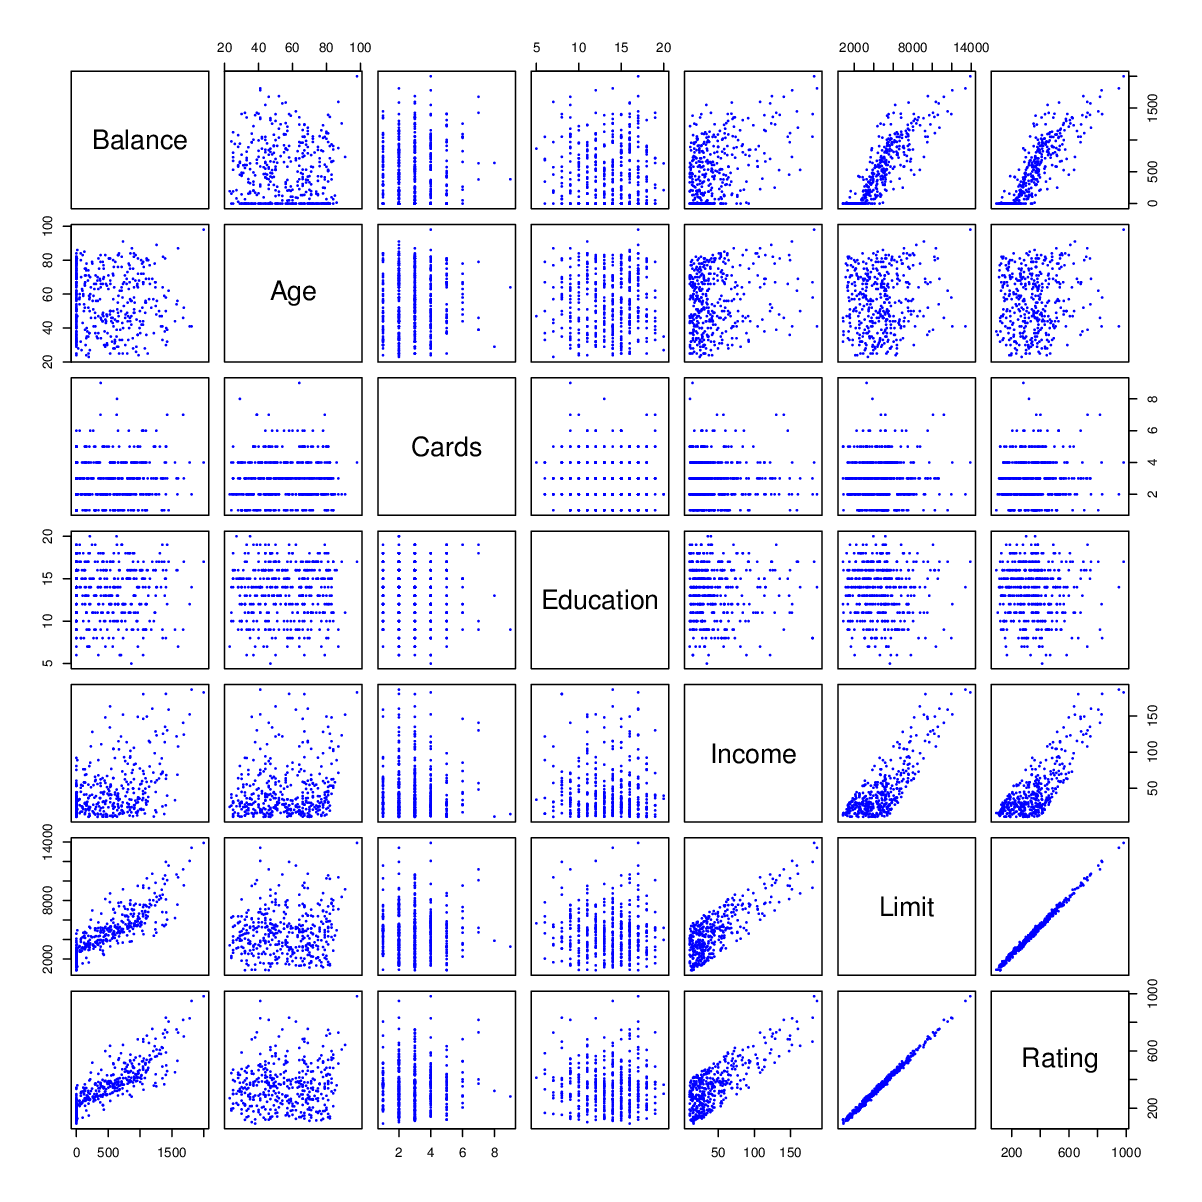
\includegraphics[width=0.95\textwidth]{3_6s}
			\end{center}
		\end{column}
	\end{columns}
	\bl{We need to somehow \e{encode} the qualitative predictors.}
\end{frame}

\begin{frame}{Qualitative Predictors with Two Levels}
	\begin{itemize}
		\item The variables \dat{gender}, \dat{student} and \dat{married} are qualitative
			predictors with two levels.
		\item Suppose we are interested in whether \dat{gender} influences \dat{balance}.
		\item We can define a \e{dummy variable} to encode the gender:
			\[
				x_i =
				\begin{cases}
					1 & \text{if $i$th person is \val{Female}} \\
					0 & \text{if $i$th person is \val{Male}} \\
				\end{cases}
			\]
		\item This results in the model
			\[
				y_i = \beta_0 + \beta_1 x_i + \epsilon_i =
				\begin{cases}
					\beta_0 + \beta_1 + \epsilon_i & \text{if $i$th person is \val{Female}} \\
					\beta_0 + \epsilon_i & \text{if $i$th person is \val{Male}} \\
				\end{cases}
			\]
	\end{itemize}
	\bl{The distinction is important for the interpretation of the model.}
\end{frame}

\begin{frame}{Qualitative Predictors with Two Levels}
	\begin{popblock}{0.8\textwidth}{Model Interpretation}
			\begin{align*}
				\beta_0 &: \text{average \dat{{\tiny balance}} among males}\\
				\beta_0 + \beta_1 &: \text{average \dat{{\tiny balance}} among females}\\
				\beta_1 &: \text{average \dat{{\tiny balance}} difference between females and males}\\
			\end{align*}
	\end{popblock}
	\begin{popblock}{0.8\textwidth}{Fit Result}
		\begin{tabular}[h]{lrrrr}
			{} & {\blue Coefficient} & {\blue Std. Error} & {\blue $t$-statistic} & {\blue $p$-value} \\
			\dat{Intercept} & $509.80$ & $33.13$ & $15.389$ & $< 0.0001$ \\
			\dat{gender[Female]} & $19.73$ & $46.05$ & $0.429$ & $0.6690$ \\
		\end{tabular}
	\end{popblock}
	\bl{The observed average difference of \$19.73 is \e{not} significant.}
\end{frame}

\begin{frame}{Qualitative Predictors with Two Levels}
	\begin{itemize}
		\item We can also encode the gender differently:
			\[
				x_i =
				\begin{cases}
					1 & \text{if $i$th person is \val{Female}} \\
					-1 & \text{if $i$th person is \val{Male}} \\
				\end{cases}
			\]
		\item This results in the model
			\[
				y_i = \beta_0 + \beta_1 x_i + \epsilon_i =
				\begin{cases}
					\beta_0 + \beta_1 + \epsilon_i & \text{if $i$th person is \val{Female}} \\
					\beta_0 - \beta_1 + \epsilon_i & \text{if $i$th person is \val{Male}} \\
				\end{cases}
			\]
	\end{itemize}
	\bl{This leads to a different interpretation of the coefficients.}
\end{frame}

\begin{frame}{Qualitative Predictors with Two Levels}
	\begin{popblock}{0.8\textwidth}{Model Interpretation}
			\begin{align*}
				\beta_0 &: \text{overall average \dat{{\tiny balance}}, disregarding gender}\\
				\beta_1 &: \text{amount  above (below) average for females (males)}\\
			\end{align*}
	\end{popblock}
	\begin{popblock}{0.8\textwidth}{Fit Result}
		\begin{tabular}[h]{lrrrr}
			{} & {\blue Coefficient} & {\blue Std. Error} & {\blue $t$-statistic} & {\blue $p$-value} \\
			\dat{Intercept} & $519.67$ & $23.03$ & $22.569$ & $< 0.0001$ \\
			\dat{gender} & $9.87$ & $23.03$ & $0.429$ & $0.6690$ \\
		\end{tabular}
	\end{popblock}
	\bl{Note that the fit is essentially the same as before.}
\end{frame}

\begin{frame}{Qualitative Predictors with more than Two Levels}
	\begin{itemize}
		\item The \dat{ethnicity} variable has three possible values.
		\item In this case we need two dummy variables for the encoding, $x_{i1}$ and $x_{i2}$. 
		\item We choose the value \val{African American} as the \e{baseline}:
			\[
				x_{i1} =
				\begin{cases}
					1 & \text{if $i$th person is \val{Asian}} \\
					0 & \text{if $i$th person is not \val{Asian}} \\
				\end{cases}
				\;\;\;\;
				x_{i2} =
				\begin{cases}
					1 & \text{if $i$th person is \val{Caucasian}} \\
					0 & \text{if $i$th person is not \val{Caucasian}} \\
				\end{cases}
			\]
		\item This results in the model
			\[
				y_i = \beta_0 + \beta_1 x_{i1} + \beta_2 x_{i2} + \epsilon_i =
				\begin{cases}
					\beta_0 + \beta_1 + \epsilon_i & \text{if $i$th person is \val{Asian}} \\
					\beta_0 + \beta_2 + \epsilon_i & \text{if $i$th person is \val{Caucasian}} \\
					\beta_0 + \epsilon_i & \text{if $i$th person is \val{African American}} \\
				\end{cases}
			\]
	\end{itemize}
	\bl{The choice of the baseline is arbitrary.}
\end{frame}

\begin{frame}{Qualitative Predictors with more than Two Levels}
	\begin{popblock}{0.8\textwidth}{Model Interpretation}
			\begin{align*}
				\beta_0 &: \text{average \dat{{\tiny balance}} among African Americans}\\
				\beta_1 &: \text{average \dat{{\tiny balance}} difference between African Americans and Asians}\\
				\beta_2 &: \text{average \dat{{\tiny balance}} difference between African Americans and Caucasians}\\
			\end{align*}
	\end{popblock}
	\vspace{-8mm}
	\begin{popblock}{0.8\textwidth}{Fit Result}
		\begin{tabular}[h]{lrrrr}
			{} & {\blue Coefficient} & {\blue Std. Error} & {\blue $t$-statistic} & {\blue $p$-value} \\
			\dat{Intercept} & $531.00$ & $46.32$ & $11.464$ & $< 0.0001$ \\
			\dat{ethnicity[Asian]} & $-18.69$ & $65.02$ & $-0.287$ & $0.7740$ \\
			\dat{ethnicity[Caucasian]} & $-12.50$ & $56.68$ & $-0.221$ & $0.8260$ \\
		\end{tabular}
	\end{popblock}
	\vspace{-3mm}
	\bl{We always need one less dummy variable than there are levels.}
\end{frame}

\begin{frame}{Extensions of the Linear Model}
	\begin{itemize}
		\item The standard linear regression model provides easily interpretable results.
		\item It also works well on many real world problems (event though the true\\
			relationships are rarely linear).
		\item However, it has the restrictive assumptions of \e{additivity} and \e{linearity}:
			\begin{cpage}
				\begin{enumerate}
					\item {\orange Additive assumption}: The effect of a predictor $X_j$ on the response $Y$
						is independent of the other predictors.
					\item {\orange Linearity assumption}: The change in the response $Y$ due to a one-unit 
						change in $X_j$ is constant.
				\end{enumerate}
			\end{cpage}
	\end{itemize}
	\bl{We explore some ways to weaken these assumptions while keeping the model linear.}
\end{frame}

\begin{frame}{Removing the Additive Assumption}
	\begin{itemize}
		\item We explore the idea of \e{interaction terms} using the \dat{Advertising} data set.  
		\item In particular, we want to check whether there is some synergy between\\
			the \dat{TV} and \dat{radio} budgets.
		\item Recall the form of the additive model only including the \e{main effects}:
			\[
				Y = \beta_0 + \beta_1 x_1 + \beta_2 x_2 + \epsilon
			\]
			\[
				\mdat{sales} = \beta_0 + \beta_1\times\mdat{TV} + \beta_2\times\mdat{radio} + \epsilon
			\]
		\item We now drop the additive assumption and introduce an interaction term:
			\[
				Y = \beta_0 + \beta_1 x_1 + \beta_2 x_2 + {\blue \beta_3 x_1 x_2} + \epsilon
			\]
			\[
				\mdat{sales} = \beta_0 
				+ \beta_1\times\mdat{TV} 
				+ \beta_2\times\mdat{radio} 
				+ {\blue \beta_3\times\mdat{TV}\times\mdat{radio}} + \epsilon
			\]
	\end{itemize}
	\bl{This model is still linear in the parameters $\bm{\beta}$. Always include the \e{main effects}.}
\end{frame}

\begin{frame}{Removing the Additive Assumption}
	\begin{itemize}
		\item We can write the model in a slightly different form.
			\begin{align*}
				Y &= \beta_0 + \beta_1 x_1 + \beta_2 x_2 + \beta_3 x_1 x_2+ \epsilon \\
				{} &= \beta_0 + {\blue (\beta_1 + \beta_3 x_2)} x_1 + \beta_2 x_2 + \epsilon \\
				{} &= \beta_0 + {\blue \widetilde{\beta}_1} x_1 + \beta_2 x_2 + \epsilon \\
			\end{align*}
			\vspace{-12mm}
			\begin{align*}
				\mdat{sales} &= \beta_0 
				+ \beta_1\times\mdat{TV} 
				+ \beta_2\times\mdat{radio} 
				+ \beta_3\times\mdat{TV}\times\mdat{radio} + \epsilon\\
				{} &= \beta_0
				+ {\blue (\beta_1 + \beta_3\times\mdat{radio})}\times\mdat{TV} 
				+ \beta_2\times\mdat{radio} 
				+ \epsilon\\
				{} &= \beta_0
				+ {\blue\widetilde{\beta}_1}\times\mdat{TV} 
				+ \beta_2\times\mdat{radio} 
				+ \epsilon\\
			\end{align*}
		\vspace{-12mm}
		\item We can now interpret $\beta_3$ as the increase of the influence of \dat{TV} due to \dat{radio} 
			(or vice versa).
	\end{itemize}
	\bl{Remember we do not make formal claims of causality.}
\end{frame}

\begin{frame}{Removing the Additive Assumption}
	\begin{popblock}{0.8\textwidth}{Fit Result ($R_\text{interaction}^2 = 0.968,\; R_\text{additive}^2 = 0.897$)}
		\begin{tabular}[h]{lrrrr}
			{} & {\blue Coefficient} & {\blue Std. Error} & {\blue $t$-statistic} & {\blue $p$-value} \\
			\dat{Intercept} & $6.7502$ & $0.248$ & $27.23$ & $< 0.0001$ \\
			\dat{TV} & $0.0191$ & $0.002$ & $12.70$ & $< 0.0001$ \\
			\dat{radio} & $0.0289$ & $0.009$ & $3.24$ & $0.0014$ \\
			$\mdat{TV}\times\mdat{radio}$ & $0.0011$ & $0.000$ & $20.73$ & $< 0.0001$ \\
		\end{tabular}
	\end{popblock}
	\bl{There is strong evidence of synergy between the two budgets.}
\end{frame}

\begin{frame}{Interactions with Qualitative Predictors}
	\begin{itemize}
		\item Interaction terms with qualitative predictors are also possible.
		\item They even have a particularly nice interpretation.
		\item We return to the \dat{Credit} data set to examine this.
		\item Suppose we want to predict \dat{sales} from \dat{income} (quantitative) and
			\dat{student} (qualitative):
			\begin{align*}
				\mdat{balance}_i &\approx \beta_0 + \beta_1\times\mdat{income}_i +
				\begin{cases}
					\beta_2 & \text{if $i$th person is a student} \\
					0 & \text{if $i$th person is not a student}
				\end{cases}\\
				&= \beta_1\times\mdat{income}_i +
				\begin{cases}
					\beta_0 + \beta_2 & \text{if $i$th person is a student} \\
					\beta_0 & \text{if $i$th person is not a student}
				\end{cases}\\
			\end{align*}
	\end{itemize}
	\bl{This amounts to fitting two parallel lines: one for students and one for non-students.}
\end{frame}

\begin{frame}{Interactions with Qualitative Predictors}
	\begin{itemize}
		\item We want to allow for the effect of \dat{income} to change, depending on whether\\
			the value of \dat{student} is \val{Yes} or \val{No}.
		\item We therefore introduce an interaction term and the model becomes:
			\begin{align*}
				\mdat{balance}_i &\approx \beta_0 + \beta_1\times\mdat{income}_i +
				\begin{cases}
					\beta_2 + \beta_3 & \text{if $i$th person is a student} \\
					0 & \text{if $i$th person is not a student}
				\end{cases}\\
				&= 
				\begin{cases}
					(\beta_0 + \beta_2) + (\beta_1 + \beta_3)\times\mdat{income}_i & \text{if $i$th person is a student} \\
					\beta_0  + \beta_1\times\mdat{income}_i & \text{if $i$th person is not a student}
				\end{cases}\\
			\end{align*}
	\end{itemize}
	\bl{The lines are no longer parallel: the slope now depends on the value of \dat{student}.}
\end{frame}

\begin{frame}{Interactions with Qualitative Predictors}
	\vspace{-10mm}
	\begin{center}
		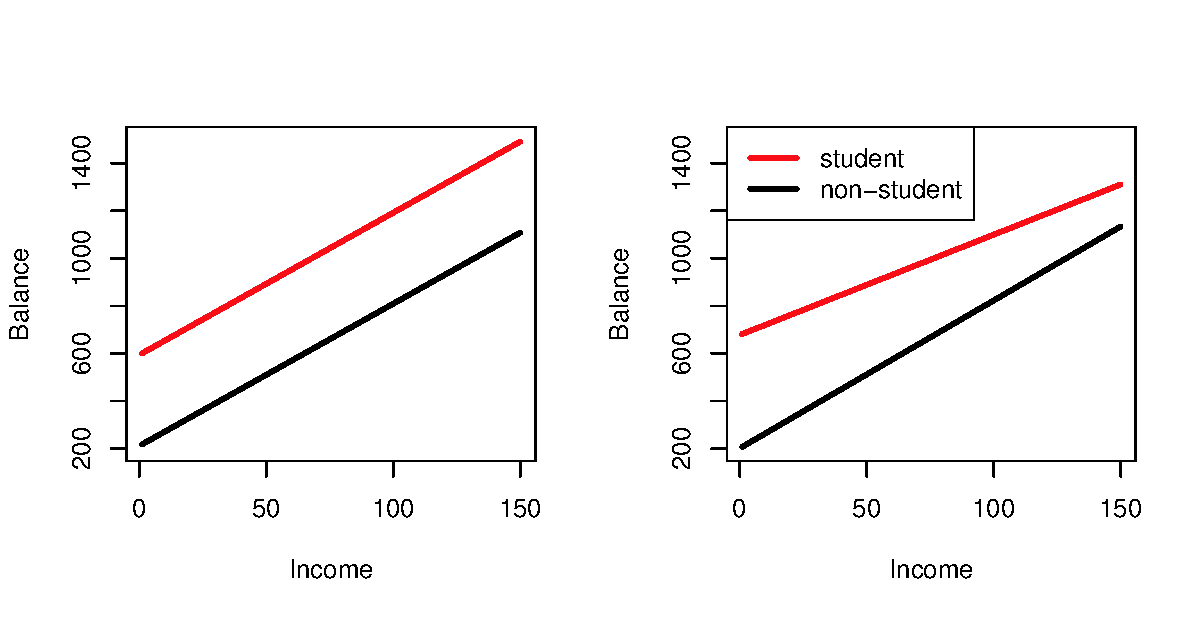
\includegraphics[width=0.8\textwidth]{3_7}
		 
		{\blue Left}: additive model, {\blue Right}: model with interaction term.
	\end{center}
	\bl{In the model with interaction the slopes are different.}
\end{frame}
\end{document}
